\documentclass[11pt]{article}
\usepackage{graphicx}
\usepackage[T1]{fontenc}
\usepackage[polish]{babel}
\usepackage{tabularx}
\usepackage[table,xcdraw]{xcolor}
\usepackage[utf8]{inputenc}
\usepackage{lmodern}
\usepackage{multirow}
\usepackage{array}
\usepackage{booktabs}
\selectlanguage{polish}
\usepackage{titlesec}
\usepackage{amsmath}
\usepackage{esint}
\usepackage{textpos}
\usepackage{chngpage}
\usepackage{calc}
\usepackage{algorithm}
\usepackage[noend]{algpseudocode}
\usepackage{placeins}
\usepackage{longtable}

\let\Oldsection\section
\renewcommand{\section}{\FloatBarrier\Oldsection}

\let\Oldsubsection\subsection
\renewcommand{\subsection}{\FloatBarrier\Oldsubsection}

\let\Oldsubsubsection\subsubsection
\renewcommand{\subsubsection}{\FloatBarrier\Oldsubsubsection}
\titlelabel{\thetitle.\quad}

\begin{document}
\begin{titlepage}
\centering

{\large Wydział Matematyki i Nauk Informacyjnych Politechniki Warszawskiej}

\vspace{1cm}

\includegraphics[scale=0.15]{logo}
\vspace{3cm}

{\Huge\bfseries Symulacja wyścigów samochodowych w 3D}

\vspace{0.5cm}

{\Large Grafika Komputerowa I}
\vspace{2cm}

{\Large Autor: \textbf{Maciej Grzeszczak}}

\vspace{1cm}

{\large v1.0}

\vspace{1cm}

\vfill

{\itshape {\large 10 grudnia 2016r.}}
\end{titlepage}

\tableofcontents


\begin{table}[!h]
\centering
\def\arraystretch{2}%
\caption{Lista zmian}

\resizebox{\textwidth}{!}{
\begin{tabular}{|p{3cm}|p{4cm}|p{6cm}|p{2cm}|}
\hline
Data                 & Autor             & Opis zmiany                                                               & Wersja                                                 \\ \hline
10.12.2016                      & Maciej Grzeszczak      & Pierwsza wersja dokumentu  & 1.0 \\ \hline
                      
\end{tabular}%
}
\end{table}


\newpage


\section{Specyfikacja}
\subsection{Opis biznesowy}

\par Niniejszy program służy do przedstawienia różnych modeli oświetlenia w grafice 3D wykorzystując do tego scenę z poruszającymi się pojazdami, które biorą udział w wyścigu. Aplikacja jest przeznaczona do użytku dla każdego. Użytkownik oprócz poruszania się pojazdem będzie mógł przełączać między poszczególnymi modelami oświetlenia, cieniowania oraz różnymi pozycjami kamery.
\subsection{Wymagania funkcjonalne}
Poniższy rysunek w postaci diagramu UML przedstawia możliwe przypadki użycia systemu przez użytkownika:
\\
\\
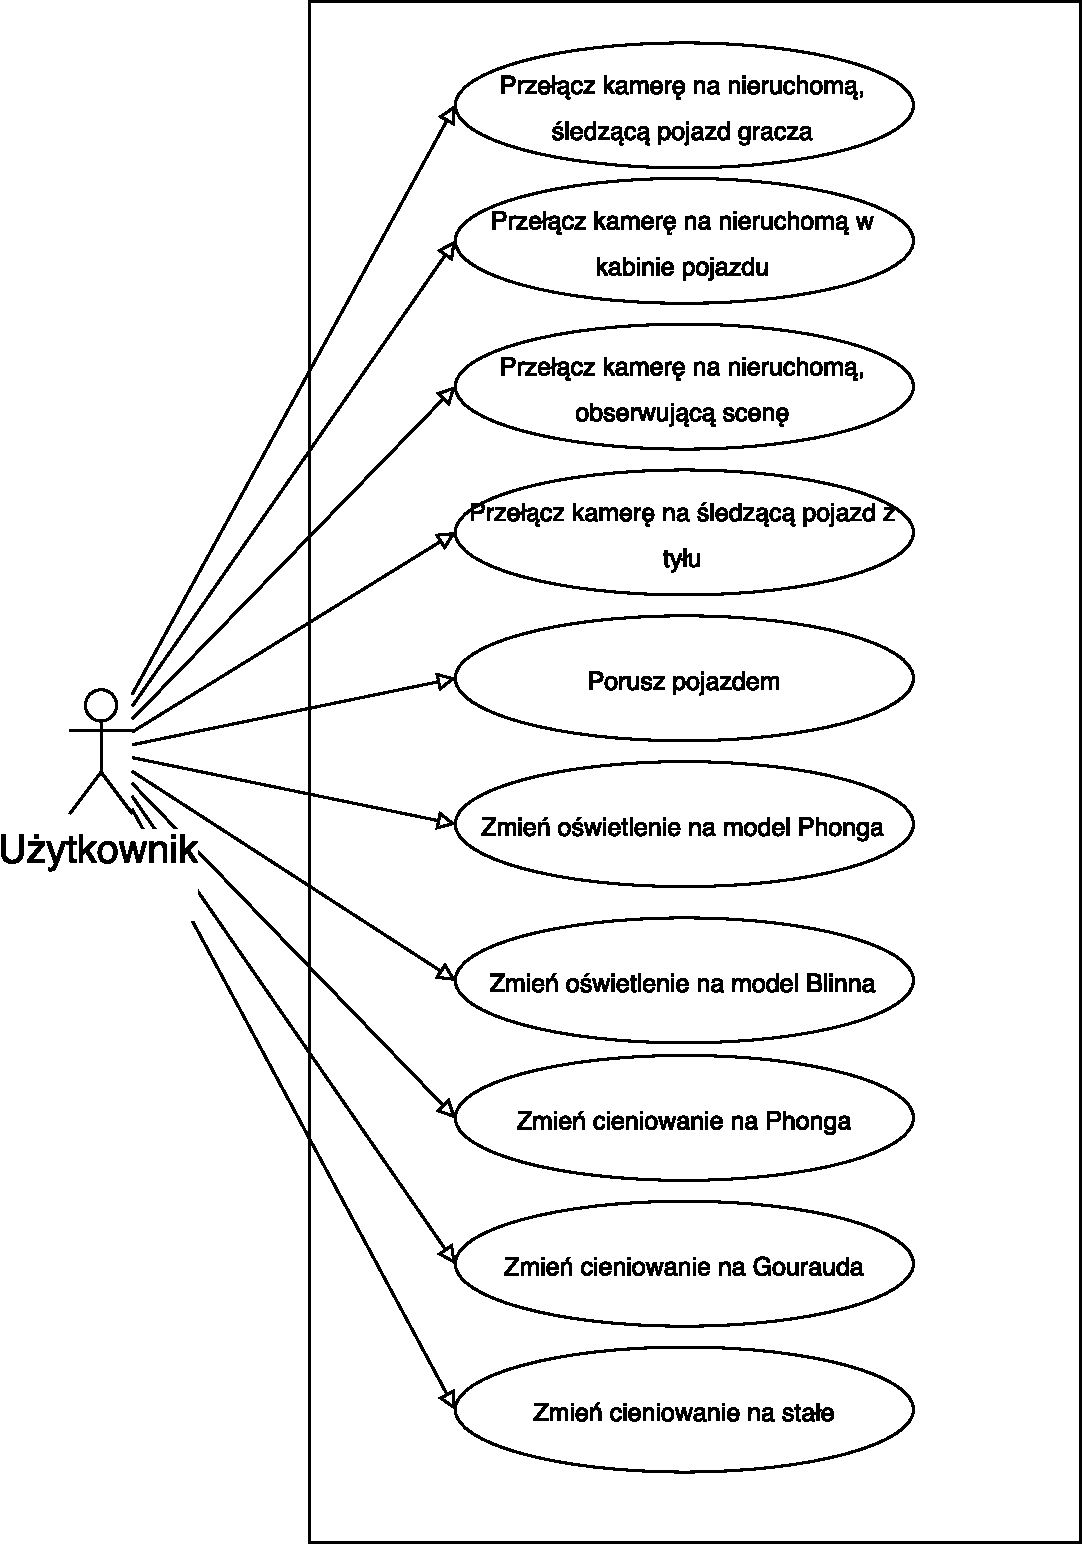
\includegraphics[scale=0.5]{use_case_pdf}

\begin{table}[!h]
\centering
\def\arraystretch{2}%
\caption{Opisy przypadków użycia dla użytkownika}

\resizebox{\textwidth}{!}{
\begin{tabular}{|p{2cm}|p{3cm}|p{6cm}|p{6cm}|}
\hline
Aktor                 & Nazwa             & Opis                                                               & Odpowiedź systemu                                                 \\ \hline
\multirow{7}{*}{Użytkownik} & Przełącz kamerę na nieruchomą w kabinie pojazdu.   & Zmiana położenia kamery na kabinę pojazdu, skierowaną na drogę przed pojazdem. & Natychmiastowa zmiana pozycji kamery.            \\ \cline{2-4} 
                      & Przełącz kamerę na nieruchomą, śledzącą scenę.       & Zmiana położenia kamery na pozycję umożliwiającą obserwowanie całej sceny z oddali.  & Natychmiastowa zmiana pozycji kamery. \\ \cline{2-4}
                      & Przełącz kamerę na śledzącą pojazd z tyłu.       & Zmiana położenia kamery na pozycję za pojazdem. Będzie się ona poruszać wraz z nim.  & Natychmiastowa zmiana pozycji kamery. \\ \cline{2-4}
                      & Porusz pojazdem.       & Przemieszczenie się pojazdu pod wpływem wciśnięcia odpowiednich klawiszy.  & Przemieszczenie się pojazdu. \\ \cline{2-4}                                            
                      & Zmień oświetlenie na model Phonga.       & Zmiana obecnego modelu oświetlenia na model Phonga.  & Natychmiastowa zmiana modelu oświetlenia na model Phonga. \\ \hline
                      & Zmień oświetlenie na model Blinna.       & Zmiana obecnego modelu oświetlenia na model Blinna.  & Natychmiastowa zmiana modelu oświetlenia na model Blinna. \\ \hline
					 & Zmień cieniowanie na Phonga.       & Zmiana obecnego trybu cieniowania na cieniowanie Phonga.  & Natychmiastowa zmiana trybu cieniowania na cieniowanie Phonga. \\ \hline
					& Zmień cieniowanie na Gourauda.       & Zmiana obecnego trybu cieniowania na cieniowanie Gourauda.  & 	Natychmiastowa zmiana trybu cieniowania na cieniowanie Gourauda. \\ \hline
					& Zmień cieniowanie na stałe.       & Zmiana obecnego trybu cieniowania na stałe.  & Natychmiastowa zmiana trybu cieniowania na cieniowanie stałe. \\ \hline
                      
\end{tabular}%
}
\end{table}



\subsection{Wymagania niefunkcjonalne}
Poniżej przykładowe wymagania niefunkcjonalne pogrupowane w poszczególne kategorie URPS.


\begin{center}

\begin{table}[!h]
\centering
\def\arraystretch{2}%
\caption{Lista wymagań niefunkcjonalnych}
\label{my-label}
\resizebox{\textwidth}{!}{
\begin{tabular}{|p{3cm}|p{0.5cm}|p{10cm}|}
\hline
Obszar wymagań &Lp & Opis                                                                                         \\ \hline
\multirow{1}{*}{Użyteczność}    & 1               & Aplikacja będzie działała na przeglądarce Mozilla Firefox dla każdej rozdzielczości powyżej 800x600. \\ \hline
\multirow{1}{*}{Niezawodność}   & 2               & Aplikacja będzie dostępna 24/7 pod podanym adresem. \\ \hline
\multirow{2}{*}{Wydajność}      
& 4               & Aplikacja będzie utrzymywać minimalny poziom 15 FPS (klatek na sekundę).  \\ \cline{2-3}
& 5 & Aplikacja będzie korzystać z biblioteki three.js która zapewni wysoką wydajność i odpowiednie zużycie zasobów.\\ \hline
\multirow{1}{*}{Utrzymanie}     
& 7               & Wraz z aplikacją zostaje dostarczona instrukcja użytkownika. \\ \hline
\end{tabular}
}
\end{table}
\end{center}

\subsection{Harmonogram projektu}

%\includegraphics[scale=0.45]{harmonogram}
%\\
%\par \noindent
\par Implementacja projektu zostanie podzielona na dwie fazy:
\begin{enumerate}
\item \textbf{Faza tworzenia sceny (7 dni)} - stworzenie świata wraz z obiektami (pojazdami), implementacja poruszania się pojazdem oraz poruszania się i zmiany pozycji kamery.
\item \textbf{Faza implementacji poszczególnych modelów oświetlenia oraz cieniowania (14 dni)} - implementacja modeli oświetlenia Phonga i Blinna oraz cieniowań: stałego, Phonga i Gourauda.
\end{enumerate}
\par \noindent

\subsection{Architektura rozwiązania}

\par Program będzie aplikacją przeglądarkową, napisaną w języku Javascript i wykorzystującą bibliotekę \textbf{three.js}, która ułatwia korzystanie z WebGL.


\end{document}